At the end of this worksheet you should be able to  
\begin{itemize}
	\item define a force and discuss the types responsible for most observable interactions
	\item add vectors graphically
	\item decompose vectors and recombine components
	\item discuss Newton's first and third law.

\end{itemize}


\begin{enumerate}
\setlength\itemsep{1 in}


\item
What is a force?

\item
How much force is 225 lbs in newtons?

\item 
How much mass in kg is 225 lbs.

\item 
Draw two vectors represented as arrows, with one of them being approximately twice as big as the other, and pointed in different directions.
\hugeskip

\item 
Graphically add these vectors up.
\hugeskip	

\item Show your results to someone else and look at their results. Draw their vector problem in the space below.
\hugeskip

\item 
A vector is described as \ang{20} \emph{north of east}. Draw a sketch of this on the coordinate plane. Also sketch in its x- and y-components. 
\giantskip

\item 
A vector is described as \ang{20} \emph{south of east}. Draw a sketch of this on the coordinate plane. Also sketch in its x- and y-components. 
\giantskip

\item 
A vector is described as \ang{20} \emph{east of north}. Draw a sketch of this on the coordinate plane. Also sketch in its x- and y-components. 
\giantskip

\item 
A vector is described as \ang{20} \emph{west of north}. Draw a sketch of this on the coordinate plane. Also sketch in its x- and y-components. 
\giantskip

\item 
Draw out your own vector in any direction on the x-y coordinate plane, and describe its coordinates from both the nearest axis, and from the positive x-axis. I have done an example of this in the space below; you do another one.

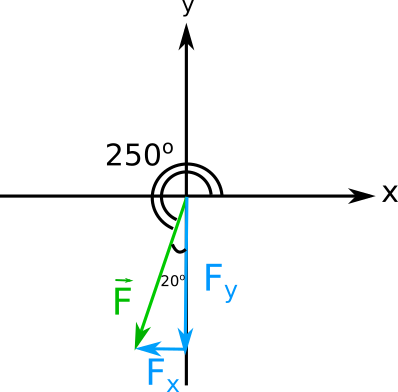
\includegraphics[width=1.75in]{week2-vector.png}\\

\item 
A force is described as being \ang{200} from the positive x direction. Express this in three other equivalent ways


\item
A force is described as being \ang{300} from the positive x direction. Express this in three other equivalent ways

\item A vector is described as being at \ang{ -30}. Where is this and describe it in two other ways.

 
\item A book is resting on a table. What forces are acting on the book? What forces are acting on the table?


\item You are holding a glass in your hand. What forces are acting on the glass.


\item A book is sliding down a table that is inclined on one side. What forces are acting on the book?


\item What are the x and y components of a \SI{100}{N} force that is acting on an object at an angle describes as \ang{20} North of West?\hugeskip

\item Vector $\vec{A}$ is \SI{10}{N} \ang{30} \emph{north of east} and vector $\vec{B}$ is 40 N \emph{east}. What is the vector sum of $\vec{A} + \vec{B}$?
\vspace{2in}

\item Use the simulation at \url{https://phet.colorado.edu/sims/html/vector-addition/latest/vector-addition_en.html} to create a vector addition problem, and work throught it with our methods to check the results.
\vspace{2in}

\item A phone is resting on an horizontal table. The phone has a weight (Force of gravity) of \SI{10}{N}. What must the normal force from the table be for there to be \SI{0}{N} \emph{net force} on the phone?\\

\item One side of the table that the phone is resting on is raised so that the surface is at a \ang{10} angle with respect to the horizontal. For this problem, make your coordinate system so that the x-axis is parallel to the surface of the table, and the y-axis is perpendicular to the table. With this coordinate system, what are the x and y components of the weight of the phone? 
\hugeskip
\hugeskip

\item From the same problem as above, what would the normal force need to be so that the net force in the y-direction is \SI{0}{N}? What would the force of friction need to be so that the net force in the x-direction is \SI{0}{N}?
\hugeskip

\item If a vector has an x-component of \SI{+10}{N}, and a y-component of \SI{+20}{N}, then what is the magnitude and direction of the vector?
\hugeskip

\item If a vector has an x-component of \SI{-10}{N}, and a y-component of \SI{+20}{N}, then what is the magnitude and direction of the vector?
\hugeskip

\item If a vector has an x-component of \SI{+10}{N}, and a y-component of \SI{-20}{N}, then what is the magnitude and direction of the vector?
\hugeskip

\item If a vector has an x-component of \SI{-10}{N}, and a y-component of \SI{-20}{N}, then what is the magnitude and direction of the vector?
\hugeskip

\item A person is pulling a sled with a rope across level snowy ground (frictionless). The sled has a weight of \SI{1000}{N}, and the person is pulling with a force of \SI{500}{N} at an angle of \ang{25} with respect to the horizontal. What are the x- and y- components of this tension force and what would the normal force need to be so that the net force is zero in the y-direction? What is the net force in the x-direction?

\end{enumerate}